\documentclass[twocolumn,11pt]{article}
\usepackage{10x23project}
\usepackage{booktabs}
\usepackage{xcolor}
\newcommand{\todo}[1]{\textcolor{red}{[TODO: #1]}}

\begin{document}

\title{Generating Urban Massing in Context from Text and Block Graphs\\[2pt]\large Midway Executive Summary}
\author{Daehong Kim \& James Fu \& Chenyue Shen\\
\texttt{\{daehongk, jfu2, chenyues\}@andrew.cmu.edu}\\
10-x23 Generative AI Course Project}
\date{\today}
\maketitle

% =====================================================================
\section{Introduction}
In early urban design, coverage, floor area ratio (FAR), height and use are fixed for each block before any building is drawn, and designers then try many massings that meet these numbers and fit the site. We frame this step as conditional generation: given a real 512\,m tile of New York City with 1--4 adjacent blocks masked out and a short request such as ``make these two blocks dense mid-rise housing'', generate several 2.5D building maps for the masked blocks that meet per-block targets and fit the surrounding city (Figure~\ref{fig:overview}). A language model turns the request into an editable table of targets, and a graph-conditioned discrete diffusion model adapted from \citet{liu2025controllable} generates the map.

At midway, the NYC dataset is complete (33,337 blocks, 84,981 samples) and the original Liu model is trained and evaluated as our first baseline. With true block centers it reproduces the street grid and block types, but its learned localization is no better than guessing inside the coarse cell it is given, and 35\% of the masked area becomes street. In a city, block outlines are known and should not be inferred, which motivates our changes. Since the proposal, we added a true-center baseline and propose a retrieval baseline and a no-GNN ablation to isolate each gain. We expect numeric attributes to lower per-block FAR and coverage error, polygon allocation to remove the localization error, and the context input to make generated blocks continuous with their surroundings.

\begin{figure*}[t]
    \centering
    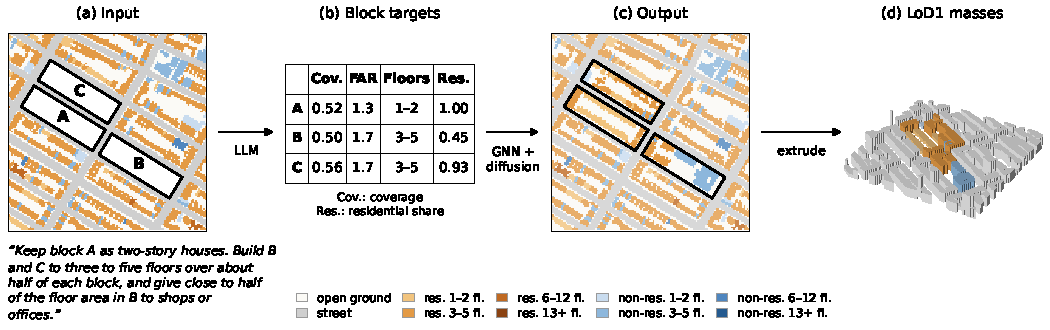
\includegraphics[width=\textwidth]{fig/overview.pdf}
    \caption{Task and pipeline on one real sample from Park Slope, Brooklyn: (a) 512\,m tile with three masked blocks and a request, (b) per-block targets from the language model, (c) blocks filled by the diffusion model (shown: the real map, i.e.\ the training target), (d) extrusion by height class.}
    \label{fig:overview}
\end{figure*}

% =====================================================================
\section{Dataset and Task}
\paragraph{Obtaining the data.} We use three NYC open datasets: PLUTO\footnote{\url{https://data.cityofnewyork.us/d/64uk-42ks}} (use, floors and FAR per tax lot), Building Footprints\footnote{\url{https://data.cityofnewyork.us/d/5zhs-2jue}} (outlines and roof heights) and Tax Lots\footnote{\url{https://data.cityofnewyork.us/d/i38t-6if2}} (lot boundaries), plus borough boundaries for the land mask. A script downloads them through the city's Socrata API; our version was downloaded on 2026-11-16 with PLUTO release 26v2, and the script records both so the dataset can be rebuilt. NYC fits our goal because heights, floor counts and land use come from official records for every building in a large, varied city, and the data is free to use.

\paragraph{Processing.} Footprints are linked to PLUTO lots; floors are roof height divided by a floor height fitted per borough on single-building lots (3.7--4.1\,m) and binned into four height classes (1--2, 3--5, 6--12, 13+ floors). Lots merged by tax block give block polygons, and for each block we compute coverage, FAR, median floors and residential share. Blocks that are under construction, too small or large, thin, or whose footprint FAR disagrees with PLUTO are flagged; they stay in the map as context but are never targets (30,866 of 33,337 blocks are valid). Block FAR from footprints matches PLUTO with $r=0.978$ on valid blocks. The city is rasterized once at 1\,m and aggregated to a 4\,m grid with 10 classes: street, open ground, and residential or non-residential buildings in the four height classes. Two blocks are connected in the block graph when they face each other across a street. A sample is a connected group of 1--4 valid blocks and a 512\,m ($128\times128$) window placed randomly around it with at least 48\,m of context. Community districts are split within each borough into train/val/test (55/5/10 district codes; park and airport codes are all in train), giving 55,813/3,825/19,380 samples after removing training samples whose context shows val or test blocks.

\paragraph{Requests.} No text is written by hand. An LLM writes requests from the true block tables in varied styles (exact numbers, vague words tied to NYC quantiles such as ``dense'' = top third of block FAR, comparisons with neighbors), and we keep requests from which a second LLM pass recovers the table. \todo{Chenyue: status and number of generated requests, parse accuracy so far.}

\paragraph{Task.} Let $x$ be the class map of a tile, $M$ the mask of the target blocks, $\mathcal{B}$ the block polygons and $s$ the request. A language model gives a target table $T = f(s, \mathcal{B}, x_{\bar M})$, and the generator samples
\begin{equation}
    \hat{x}_M \sim p_\theta\left(x_M \mid x_{\bar M}, M, \mathcal{B}, T\right).
\end{equation}
The map outside $M$ is fixed, and samples for one input should differ while meeting $T$. The generator is trained with true tables and tested with both true and parsed ones.

\paragraph{Metrics.} \emph{Condition error}: per-block absolute error in coverage and FAR, and accuracy of the dominant height class and use. FAR is computed from the map with one floor count per height class fitted on training blocks; because four height classes cannot encode exact floors, even the real map has a FAR error of 0.22 (median relative error 9\%), which we report as an oracle row. \emph{Fit with the surroundings}: share of generated building cells on street cells (Out-Block, \citealp{he2023globalmapper}) and how close height differences across the mask boundary are to those of real tiles. \emph{Realism}: accuracy of a small CNN trained to separate real from generated target regions (50\% is best), and distances between distributions of footprint measures \citep{fleischmann2019momepy}, computed per connected building region because adjacent row houses merge at 4\,m (33 buildings per block become 11 regions on average). \emph{Diversity}: share of cells that differ between two of four samples for one input. All metrics are computed inside $M$ on a fixed random ordering of test samples, with 95\% bootstrap intervals over blocks, because overlapping windows share blocks.

% =====================================================================
\section{Related Work}
Scene-graph conditioning began with images \citep{johnson2018sg2im}. \citet{liu2025controllable} extend it to 3D outdoor scenes with a graph attention network \citep{velickovic2018gat}, a module that places node embeddings on a bird's-eye-view grid, and discrete diffusion \citep{hoogeboom2021argmax,austin2021d3pm}. They also turn text into the graph with an LLM, as our request step does. Their nodes are objects in synthetic driving scenes whose positions must be inferred; in a city, block outlines are known, which motivates our second change.

Learning-based urban layout generation began with single blocks. BlockPlanner \citep{xu2021blockplanner} and GlobalMapper \citep{he2023globalmapper} generate the buildings of one block from its shape with graph-based models, so neighboring blocks can look unrelated. COHO \citep{he2024coho} generates city-scale layouts with heights, and CityDreamer \citep{xie2024citydreamer} generates unbounded semantic and height maps. None of them lets a user set the density or use of a block.

Work in architecture and planning adds design targets. Text-to-City \citep{zhuang2024texttocity} conditions Stable Diffusion on a density token and fails when several indicators are given together. GenFusion \citep{gao2025genfusion} conditions diffusion on FAR and building density for one site. \citet{jang2026context} inpaint one site's footprint from image channels of roads, sidewalks and neighbors, without density targets, and CoMa \citep{maslov2026coma} generates one parcel's massing from its context with a vision-language model. Our task combines what these works do separately: several blocks at once, inside a real context, each with its own numeric targets, through a table the user can edit. Because \citet{jang2026context} show that context as image channels is effective without a graph, we add a no-GNN ablation to test what the graph contributes once context is given as an image.

% =====================================================================
\section{Approach}
\paragraph{Baseline: the original Liu model.} We use the 2D stage of the released code of \citet{liu2025controllable}\footnote{\url{https://github.com/yuhengliu02/control-3d-scene}} with its architecture and hyper-parameters, changing only what the data requires. \emph{Graph}: each block in the window is a node whose 27-d feature is a one-hot class label (dominant use $\times$ height class, 10 classes; empty blocks are ``open'') and Liu's coarse position code (one-hot over a $4\times4$ partition of the window plus one slot); road types are dropped. Edges connect each block to its 4 nearest blocks by centroid (street-facing edges belong to our first change). Blocks with fewer than 20 visible cells are dropped unless they are targets. \emph{Model}: a 2-layer GAT (hidden 32, 4 heads) gives each node an embedding, concatenated with the graph mean and projected to 32 channels; the allocation module writes each embedding into the single cell of the node's center, giving a $32\times128\times128$ condition map; a multinomial diffusion model \citep{hoogeboom2021argmax} with 100 steps, a cosine schedule and Liu's 3D-convolution U-Net (59.0M parameters in total) denoises the class map. \emph{Training}: loss $=0.6\,L_\text{diff}+0.2\,L_\text{edge}+0.2\,L_\text{class}$, where the GNN also reconstructs edges and classifies nodes; true centers are used for allocation, 30\% of position codes are masked, and the condition is dropped for 10\% of samples. We use AdamW, learning rate $4\times10^{-3}$ and batch 16 as Liu do, add gradient clipping at norm 1.0 after an unclipped run diverged in its second epoch, and give every model the same 12-hour budget on one A10G (55 epochs). A localization head is then post-trained for 1 hour with all other weights frozen (cross-entropy over the 16,384 cells). \emph{Sampling}: centers are drawn from the head with Gumbel noise ($\tau=2$), collisions are moved by 5 cells, and 100 denoising steps generate the full tile, which we evaluate inside $M$.

\paragraph{Main method: three changes.} \emph{(1) Numeric attributes and street-facing graph}: each node also gets coverage, FAR, median floors, residential share and area (true values for context blocks, the table for target blocks, with a flag for blocks that failed validity checks), and edges connect blocks that face each other across a street, with street width and facing length as edge features. \emph{(2) Polygon allocation}: instead of a learned center, each node embedding is written into every cell of its known polygon, and street cells get one learned embedding; the localization head is removed. \emph{(3) Context input}: the diffusion model receives the real map outside $M$ and the mask as extra channels, and noise and loss apply only inside $M$. Network, noise schedule and training settings stay as in the baseline. Cells are extruded by height class in place of Liu's 3D stage.

\paragraph{Request to table.} A prompted LLM (Qwen3-8B, no training, few-shot examples from training districts) reads the request with the target blocks and the true values of the surrounding blocks, and returns a JSON table of coverage, FAR, height class and residential share per target block.

\paragraph{Other baselines.} \emph{Liu + true centers}: the baseline with true block centers at sampling, which isolates the localization error. \emph{GlobalMapper} \citep{he2023globalmapper}: we replicate it on its released 10K-block sample and compare with the published numbers, then retrain it on NYC, rasterize its output to our grid and compare on realism, Out-Block and continuity (it has no heights or targets). \emph{Retrieval} (proposed): copy the layout of the training block with the closest targets and area, warped to the target polygon, as a check that generation beats copying. \emph{No-GNN} (proposed): change (3) with the GNN removed and the raw targets painted into block polygons as channels, as in \citet{jang2026context}.

% =====================================================================
\section{Experiments}
\begin{figure*}[t]
    \centering
    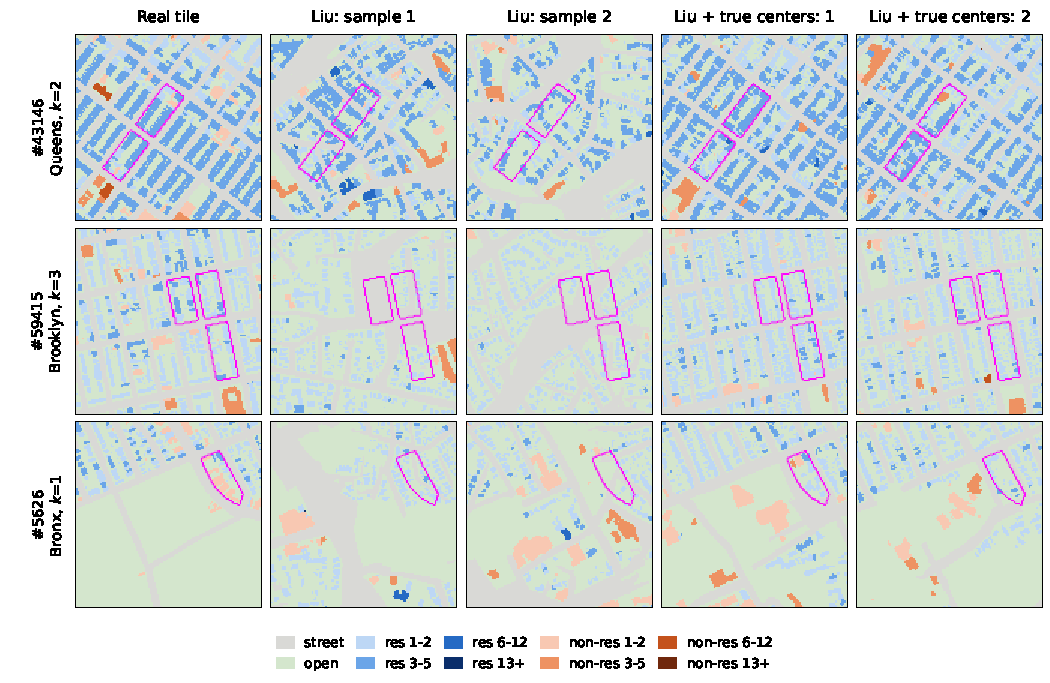
\includegraphics[width=\textwidth]{fig/baseline_samples.pdf}
    \caption{Baseline samples on held-out test districts (magenta: target blocks; the model generates the whole tile and is scored inside the outline). With learned centers (columns 2--3), misplaced blocks leave large areas that the model fills with street. With true centers (columns 4--5), the same model reproduces the street grid and row-house pattern of \#43146 and \#59415. In \#5626 the large park is one node with no size, so buildings are spread over it.}
    \label{fig:samples}
\end{figure*}

\begin{table}[t]
\centering\small
\setlength{\tabcolsep}{4pt}
\begin{tabular}{lcc}
\toprule
Metric (inside $M$) & Liu & Liu + true centers \\
\midrule
Cell accuracy $\uparrow$ & 0.317 {\scriptsize[.301,.333]} & 0.417 {\scriptsize[.402,.432]} \\
Building / not $\uparrow$ & 0.554 {\scriptsize[.539,.568]} & 0.594 {\scriptsize[.584,.603]} \\
Height class acc. $\uparrow$ & 0.760 {\scriptsize[.715,.804]} & 0.861 {\scriptsize[.824,.897]} \\
Use acc. $\uparrow$ & 0.782 {\scriptsize[.739,.825]} & 0.863 {\scriptsize[.821,.901]} \\
Coverage error $\downarrow$ & 0.278 {\scriptsize[.262,.296]} & 0.118 {\scriptsize[.107,.130]} \\
Street cells in $M$ $\downarrow$ & 0.350 {\scriptsize[.334,.366]} & 0.107 {\scriptsize[.098,.117]} \\
Diversity & 0.610 & 0.536 \\
\bottomrule
\end{tabular}
\caption{Baseline results on the first 200 test samples (4 samples each), with 95\% bootstrap intervals over samples. Height class and use are the dominant class of building cells; the real value of street cells in $M$ is 0.}
\label{tab:baseline}
\end{table}

\paragraph{Baseline results.} Table~\ref{tab:baseline} and Figure~\ref{fig:samples} show the original Liu model on the first 200 samples of our fixed test ordering (77/50/47/26 samples with 1/2/3/4 target blocks). We believe these numbers are correct for three reasons. First, before full training the pipeline memorized 8 tiles (cell accuracy 100\% with true centers, 93\% with learned ones), so data, model and sampling are wired correctly. Second, the diffusion loss converged (6.1 in epoch 1 to 4.20 in epoch 55, flat after epoch 40) with a stable gradient norm. Third, the gap between the two columns matches what the localization head can know: its final loss of 7.07 is no lower than $\ln 1024 = 6.93$, the loss of guessing uniformly inside the $128\times128$\,m cell given by the position code, so it learns almost nothing beyond that code, and a 4\,m error in a block's center misplaces its whole embedding. Height class and use are high in both columns because they are given as the node label; only 68\% of building cells in a real block share the block's label, which bounds what one label can describe. Cell accuracy stays below 0.42 even with true centers because the model knows nothing about block size or shape, and the context it draws is invented (Figure~\ref{fig:samples}). Training took 12\,h, post-training 1\,h, and sampling 0.47\,s per tile.

\begin{table*}[t]
\centering\small
\begin{tabular}{l|cccc|cc|cc|c}
\toprule
& \multicolumn{4}{c|}{Condition} & \multicolumn{2}{c|}{Surroundings} & \multicolumn{2}{c|}{Realism} & \\
Model & FAR err.$\downarrow$ & Cov. err.$\downarrow$ & Height acc.$\uparrow$ & Use acc.$\uparrow$ & Out-Block$\downarrow$ & Boundary$\downarrow$ & CNN acc.$\to$50\% & Footprint dist.$\downarrow$ & Diversity \\
\midrule
Real map (oracle) & 0.22 & 0 & 1 & 1 & -- & -- & 50\% & 0 & -- \\
Retrieval (proposed) & & & & & & & & & \\
GlobalMapper & n/a & n/a & n/a & n/a & & & & & \\
Liu & & & & & & & & & \\
Liu + true centers & & & & & & & & & \\
\quad + (1) numeric attributes, street graph & & & & & & & & & \\
\quad + (2) polygon allocation & & & & & & & & & \\
\quad + (3) context input (full model) & & & & & & & & & \\
Full model without GNN (proposed) & & & & & & & & & \\
\bottomrule
\end{tabular}
\caption{Main comparison (skeleton) on the test districts with true target tables. Rows (1)--(3) are cumulative. Boundary is the distance between distributions of height differences across the mask boundary in generated and real tiles.}
\label{tab:main}
\end{table*}

\paragraph{Planned experiments.} Our research question is whether a scene-graph diffusion model can meet numeric targets for several blocks at once while fitting a real neighborhood, and which part of the pipeline limits it. Table~\ref{tab:main} compares all generators with true tables. Its rows answer four sub-questions. (Q1) Do numeric attributes lower FAR and coverage error? We expect yes, since the baseline graph cannot express density. (Q2) Does polygon allocation help beyond knowing the center? Comparing (2) with \emph{Liu + true centers}, rather than with Liu, separates the value of the shape from the value of the position. (Q3) Does the context input make blocks continuous with their surroundings? We expect lower Boundary and Out-Block, and better realism than GlobalMapper, which sees one block at a time. (Q4) Does the graph still help once context is an image? The full model against its no-GNN version answers this; if they are close, the graph's main value is as the interface to the language model. Table~\ref{tab:llm} runs the full model with true and with parsed tables to split the remaining condition error between the two steps; we expect most of it to come from generation. A planned plot shows generated against target FAR per block for the baseline and full model, colored by height class, since our dataset has few 13+ blocks (4 in the first 200 test samples) and errors there need separate reporting. Table~\ref{tab:gm} records the GlobalMapper replication.

\begin{table}[t]
\centering\small
\begin{tabular}{lccc}
\toprule
Full model with & FAR err. & Cov. err. & Height acc. \\
\midrule
True table & & & \\
Parsed table (Qwen3-8B) & & & \\
\bottomrule
\end{tabular}
\caption{Error split between the language and generation steps (skeleton).}
\label{tab:llm}
\end{table}

\begin{table}[t]
\centering\small
\begin{tabular}{lcccc}
\toprule
& L-Sim$\uparrow$ & Overlap$\downarrow$ & Out-Block$\downarrow$ & FID$\downarrow$ \\
\midrule
Published & 22.45 & 1.42\% & 0.89\% & 14.94 \\
Ours (10K sample) & \todo{} & & & \\
\bottomrule
\end{tabular}
\caption{GlobalMapper replication \citep{he2023globalmapper}. \todo{Chenyue: fill or report status.}}
\label{tab:gm}
\end{table}

% =====================================================================
\section{Plan, Human Work and AI Use}
\paragraph{Timeline.} \textbf{Done}: NYC dataset and QA (Daehong, Nov 16); baseline adapter, overfit test, training and evaluation of Liu and Liu + true centers (James, Nov 18). \textbf{Nov 20}: team decisions on test-set size (1,000--2,000 samples), retrieval and no-GNN baselines; evaluation code with all Table~\ref{tab:main} metrics (Daehong); request generation and GlobalMapper replication (Chenyue) \todo{confirm}. \textbf{Nov 21--26}: train changes (1), (2), (3) on the A10G, about 13\,h each, coding the next change while the previous one trains (James; Daehong pair-programs (2) and (3)); LLM step evaluated on the val districts (Chenyue). \textbf{Nov 27}: retrieval and no-GNN runs if approved (James, Daehong). \textbf{Dec 1}: GlobalMapper on NYC (Chenyue); full Tables~\ref{tab:main}--\ref{tab:llm} (all). \textbf{Dec 4 / Dec 10}: poster; final report and code (all). If time runs short, we drop the no-GNN run before any of the three changes.

\paragraph{Human work.} The team chose the task, data and metrics, defined the block, sample and split rules, and made each design decision in the pipeline (e.g.\ validity flags, the 20-cell sliver filter after James noticed context blocks cut by the window edge in the graph plots, gradient clipping after the first run diverged, and the true-center baseline after questioning why a known position should be learned). The team reads every result figure and checks dataset statistics against PLUTO. \todo{Daehong, Chenyue: add your human-only parts.}

\paragraph{AI use so far and how we checked it.} James used an AI coding assistant (Claude Code) to write the baseline adapter, training and sampling options, monitoring scripts and a data audit, and to run the AWS jobs under his instructions. We checked this work with (i) figures of every adapter output overlaid on the real map, which revealed the sliver nodes; (ii) the 8-tile overfit test; (iii) checksums of the uploaded data; (iv) a scripted health check of the training log every 30 minutes; and (v) audit numbers cross-checked against the dataset's QA report. Each change is a separate commit with a description, so it can be reviewed. \todo{Daehong, Chenyue: your AI use and checks.}

\paragraph{AI use from now on.} We will use the coding assistant for the three changes and the evaluation code, and check each change with the same overfit test and with metrics on the real map (which must give the oracle row of Table~\ref{tab:main}). LLMs are also part of the method, where they write and parse requests; we read a random set of 50 requests and parsed tables each week to catch failures the metrics miss. All analysis and conclusions are written and checked by us.

% =====================================================================
\section{Thought-Experiment on Compute}
\paragraph{Compute used.} All training runs on one AWS g5.xlarge (NVIDIA A10G, 24\,GB, 4 vCPUs; \$1.006/h on demand). So far the baseline used about 15 GPU-hours: 12\,h of training, 1\,h of post-training, 0.2\,h of sampling and about 1.5\,h for the overfit test, timing and two aborted runs, i.e.\ about \$15. The dataset was built on a laptop CPU. \todo{instance uptime incl.\ idle; Chenyue's GPU use for GlobalMapper and Qwen3-8B.} We project about 80 GPU-hours (\$80) for the whole project: four NYC models at 13\,h each, GlobalMapper, and evaluation.

\paragraph{With \$1,000 of credits.} Our current results come from one seed per model, a 200-sample test subset and a 12-hour budget, all set by one GPU. With \$1,000 we would (a) run three seeds of every learned model on parallel g5 instances, so that differences in Table~\ref{tab:main} include training variance (about 160\,h, \$160); (b) evaluate on all 19,380 test samples, which takes about 11\,h per model, and on a tall-building subset (about 90\,h, \$90); (c) sweep the learning rate and training budget of the full model, since we kept Liu's settings (about 130\,h, \$130); (d) train the baseline and full model at 2\,m resolution, which separates more row houses but costs about 4$\times$ more (about 100\,h, \$100); and (e) compare Qwen3-8B with a 32B parser on a 4-GPU g5.12xlarge (about 30\,h at \$5.67/h, \$170). This totals about \$650 and leaves a margin for reruns. With only \$450, we would keep (a), (b) and part of (c), since seeds and the full test set decide whether our conclusions hold.

\bibliographystyle{plainnat}
\bibliography{references}

\end{document}
